\subsection{Product perspective}
The S2B will be used by two kinds of users: customers and store owners, and offers to each of them different functionalities:
%TODO: probably move it to product functions and write some general description here about what slides say:
% Describes external interfaces: system, 
% user, hardware, software; also 
% operations and site adaptation, and 
% hardware constraints
\subsubsection{Customer}
The customer can create reservations for a desired store: such reservation is then inserted into a queue.\\This queue is managed in order to avoid overcrowding. To achieve this, statistics about visits' durations are exploited, taking also into account information that customers may provide (e.g. which department of the store they want to visit).\\
There are multiple types of reservations that can be requested:
\begin{enumerate}
	\item Immediate reservation: the costumer wants to queue up immediately to a store. He/she is also provided with an estimation of the time he has to wait before his/her turn.
	\item Future reservation: the costumer wants to book a future visit at a desired time and store.\\ When creating the reservation the customer can specify how long he/she intends to stay and which departments of the market he/she plans to go to, in order to provide a better plan. If he/she does not specify the duration the system can infer it using some statistic built on his/her previous visits. Then the customer will be provided whit the actual time he will be able to access the store (considering the bookings from other customers).
	\item On premise reservation: the customer is allowed to enqueue directly at the store. Each of them will provide a system to print tickets so that those who do not have access to the required technology for the previous options can still line up. These tickets contain a reservation number and an estimation of the waiting time before being able to enter.
\end{enumerate}
Customers who requested an immediate or a future reservation receive an alert when they need to depart to reach the store.
This alert is based on the location of the customer, so that the time needed to reach the store is taken into account. If, for any reason, a customer cannot to go to a store he/she has lined up to it is possible for him/her to delete the immediate or future reservation. For obvious reasons the on premise reservation cannot be deleted.\\\\
Reservations can be in one of the following states:
\begin{itemize}
	\item Pending: customer cannot yet access the store
	\item Authorized: customer can access the store
	\item Current: customer is in the store
	\item Expired: customer has exited the store
\end{itemize} 
\subsubsection{Store owner}
The store owner can
\begin{enumerate}
	\item Register a store to the system so that it can be accessed by customers
	\item Set the maximum occupation threshold for each of his stores.
	\item Monitor the number of customers inside at any time
	\item Visualize statistics about the flow of clients and department occupation
\end{enumerate}
When setting the maximum occupation of a store, the owner can specify a threshold for each department or for the whole store. In the latter case the occupation of each department is set to the same value. In case customers select which section of the store they intend to visit their presence will be considered only in those specific department, in order to allow more customers in, provided that they will not come in contact with each other. For safety, if customers don't specify anything they are supposed to visit each department.
\begin{figure}[!htb]
\centering
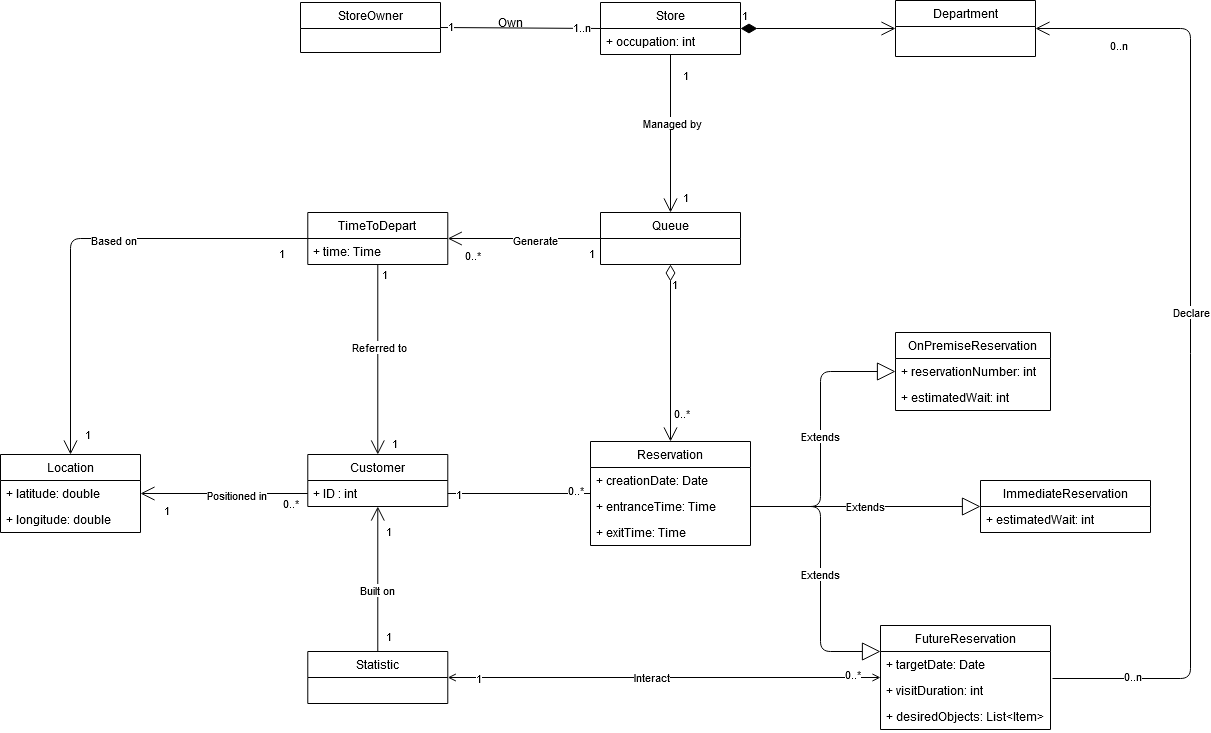
\includegraphics[width=\textwidth]{Images/ClassDiagram.png}
\caption{\label{fig:metamodel2}Class Diagram.}
\end{figure}
\newpage
\subsubsection{State charts}
Here we show the main processes that the system will manage, and the states in which the system will find itself.
\begin{figure}[!htb]
	\centering
	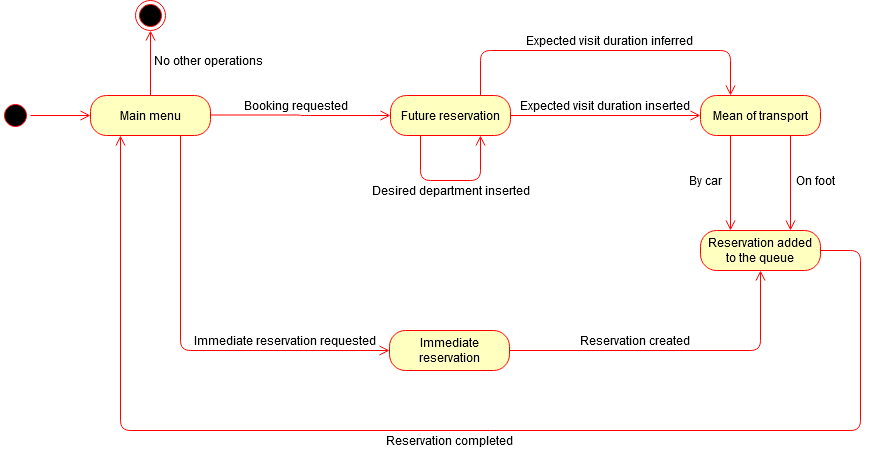
\includegraphics[width=\textwidth]{Images/StateDiagram1.png}
	\caption{\label{fig:metamodel3}State Diagram 1: Creation of a reservation.}
\end{figure}\\
%TODO add by car/on foot request
The figure above illustrates how the customer creates a reservation (virtual customer). The customer accesses the main menu. From there he/she can request an immediate reservation or a future reservation. If he/she requests an immediate reservation, it is created and the process terminates. If he/she requires a future reservation he can add the departments he/she intends to visit, and how much time he/she is going to spend at the store. Then the reservation is created and the process terminates.\\\\\\\\

\begin{figure}[!htb]
	\centering
	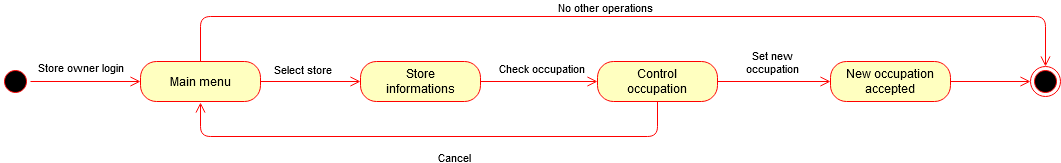
\includegraphics[width=\textwidth]{Images/StateDiagram2.png}
	\caption{State Diagram 2: Store owner sets occupation.}
\end{figure}
The figure above illustrates how the store owner sets the maximum occupation of one of his stores. The store owner logs in and is provided a main menu. He/she selects one of his stores, and is presented with the current maximum occupation of his selected store. He can change it to a value to his liking, or go back to the main menu.

\begin{figure}[!htb]
	\centering
	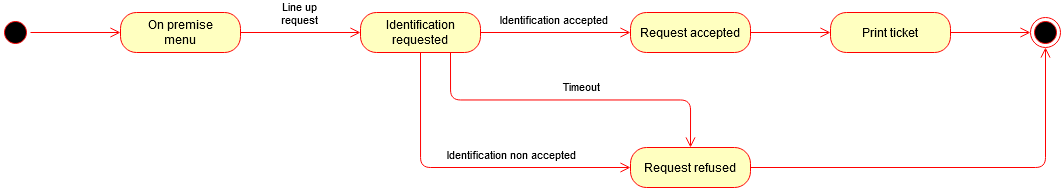
\includegraphics[width=\textwidth]{Images/StateDiagram3.png}
	\caption{State Diagram 3: On premise creation of a reservation.}
\end{figure}
The figure above illustrates how a customer can queue up on premise (physical customer). The customer is presented with an on premise main menu. From there he/she can request to queue up (create a reservation) immediately. He will be prompted to identify himself (e.g. social security card). Once identified the customer will be provided a ticket with a number that represents his position in queue and an estimate of the waiting time.

\begin{figure}[!htb]
	\centering
	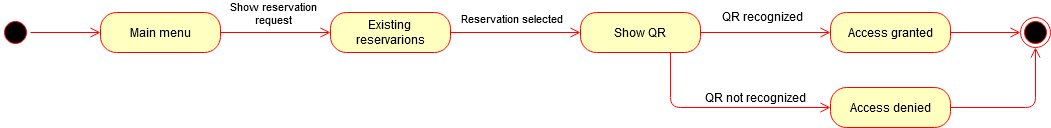
\includegraphics[width=\textwidth]{Images/StateDiagram4.png}
	\caption{State Diagram 3: Customer enters a store.}
\end{figure}
The figure above illustrates how a customer who is authorized can access the store. At the entrance of his/her store of choice he is enabled to demonstrate his authorization. Once he/she does, he is allowed to enter the store.

\subsection{Product functions}
We describe here functions that the system will support.
\begin{enumerate}
	\item Customers can queue up virtually or physically, immediately or in the future at one of the stores registered to the service.
	\item Customers can delete a virtual reservation.
	\item Customers can access the desired store when its occupation reaches acceptable levels.
	\item Customers that queued up virtually can be notified when it is time for them to depart to reach the store.
	\item Store owners can monitor the occupation in each of their stores.
	\item Store owners can define the maximum occupation of each department of their stores.
	\item Store owners can register stores to the system.
\end{enumerate}

\subsection{User characteristics}
\begin{enumerate}
	\item {\bfseries Customers}: a physical person that needs to access any of the stores registered to the system. The customers belong to all demographics, thus the need for a user-friendly interface for both virtual and physical customers. The customer needs a reasonably precise estimate of waiting time and time to get to the store.
	\item {\bfseries Store owners}: a physical or legal person that owns any number of stores and needs to enable customer access through a queue system.
\end{enumerate}

\subsection{Assumptions, dependencies and constraints}
\subsubsection{Domain Assumptions}
\begin{enumerate}[label=D\arabic*]
	\item The stores have QR activated turnstiles.
	\item Turnstiles let one and only one person in each time they unlock.
	\item Outside stores is a social security card activated ticket printer.
	\item Outside stores there is a monitor.
	\item There is no way for a customer to enter a store except from entrance and exit.
	\item Each customer has either a telephone number or an identification document.
	\item When provided, user location has maximum error of 5 meters.
	\item To register to the S2B users must have either a smartphone or a computer.
	\item To register and use the S2B users must have an internet connection.
\end{enumerate}